\section{Möglichkeiten zur Genauigkeitssteigerung
\label{perturbation:section:weitereverbesserungen}}
\rhead{Weitere Verbesserungen}
In diesem Abschnitt diskutieren wir Verbesserungsmöglichkeiten, um den Fehler weiter zu minimieren. 
Abbildung \ref{error} zeigt, dass der Fehler stark von der Intervalllänge abhängt. 
Eine Reduktion der Intervallänge beschreiben wir im nächsten Abschnitt. Weiter lassen sich mit Hilfe der Störungstheorie höherer Ordnung genauere Resultate erzielen.

\subsection{Reduktion der Intervalllänge}
In Abbildung \ref{error} ist der Fehler für die Intervalllänge von einer Sekunde ersichtlich. 
Wie man erkennen kann, nimmt dieser innerhalb wenigen Millisekunden stark zu. 
Dies ist vor allem unserem Beispiel geschuldet, da die Störung (in unserem Beispiel der Luftwiderstand) kurzfristig eine grosse Auswirkung auf das Resultat hat. 
Bei Berechnungen von z.B. Satellitenbahnen wäre dies anders, da Störungen, wie die Gravitation von Planeten, viel kleiner sind und die Abweichungen erst bei längeren Intervalldauern auftreten.

Für unser Beispiel haben wir in einem ersten Schritt die Intervallänge halbiert und sind auf die Resultate in Abbildung \ref{errorShortInterval} gekommen. 
Wie ersichtlich ist, ist der Fehler um ca. Faktor 4 kleiner. 
Wir erhalten somit weitere 2 Bit Genauigkeitsgewinn. 
Weiter ist zum Zeitpunkt $t=17s$ eine kleine numerische Instabilität beobachtbar.

\begin{figure}
    \centering
    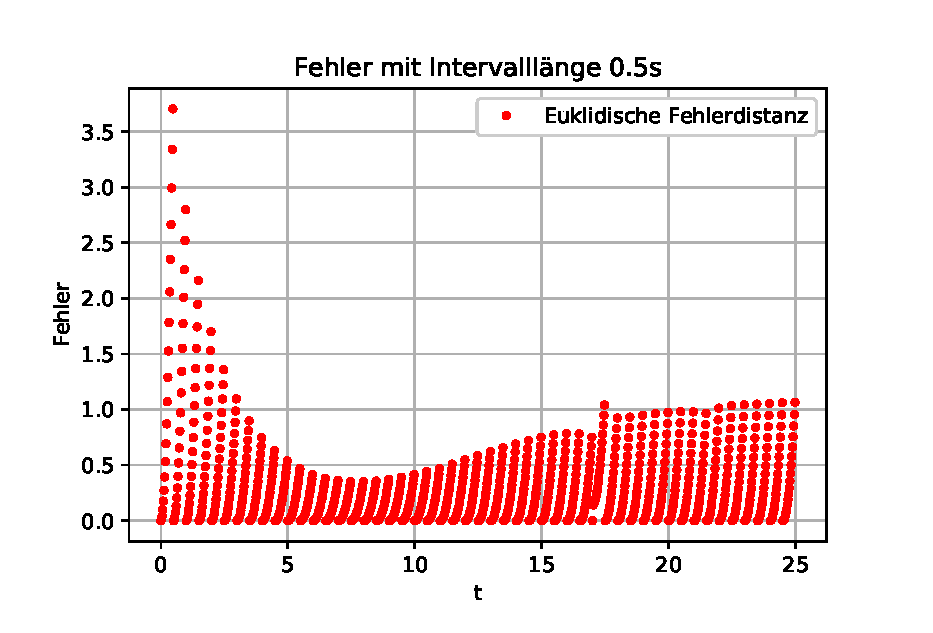
\includegraphics[scale=0.7]{papers/perturbation/bilder/perturbation_fig4.eps}
    \caption{Fehler bei halbierter Intervalldauer}
	\label{errorShortInterval}
\end{figure}

In einem zweiten Schritt haben wir die Intervallänge nochmals auf die Länge $\Delta t = 0.25$ halbiert. 
Dies ist in Abbildung \ref{errorShortInterval2} ersichtlich. 
Wir erhalten wieder einen Genaugikeitsgewinn um den Faktor 4 bzw. 2 Bit. 
Dies lässt sich leider jedoch nicht weiter beliebig fortsetzen. 
Die Rechenlast des Satelliten bleibt konstant und ist nicht von der Intervalllänge abhängig. 
Der Aufwand für die Bodenstation nimmt jedoch zu. 
Da die numerischen Berechnungen für aufwänderige Formeln (wie Satellitenbahnen) oft ein wenig dauern und gegebenfalls viel Rechenleistung benötigen, sind diese nicht günstig und können nicht beliebig oft ausgeführt werden.

\begin{figure}
    \centering
    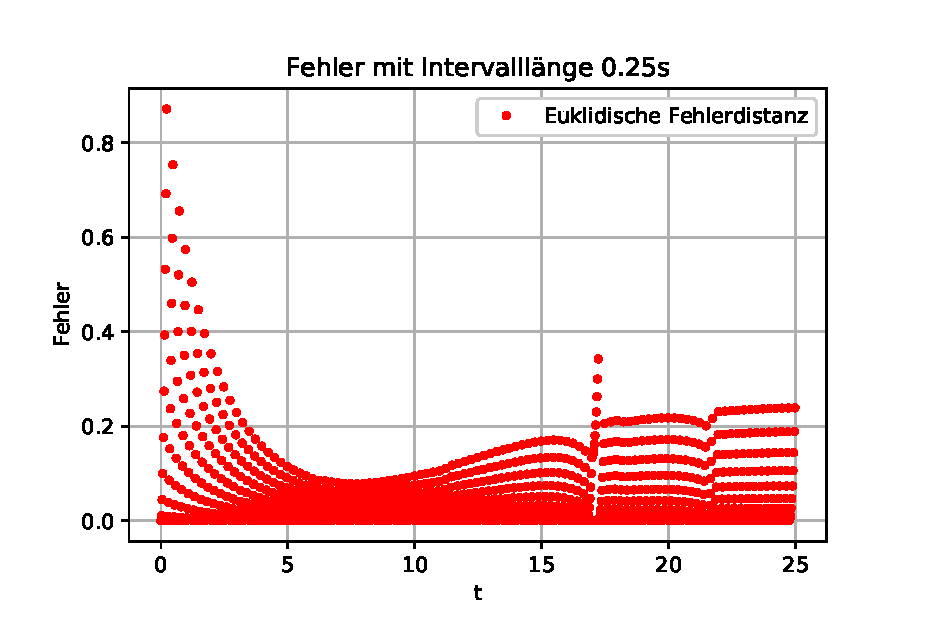
\includegraphics[scale=0.7]{papers/perturbation/bilder/perturbation_fig5.eps}
    \caption{Fehler mit einem Viertel der Intervalldauer}
	\label{errorShortInterval2}
\end{figure}

\subsection{Erhöhung der Ordnung}
Eine andere Möglichkeit zur Steigerung der Genauigkeit eröffnet sich dadurch, dass man anstelle $x_0, y_0, v_{0x}$ und $v_{0y}$, was an sich Polynome nullter Ordnung sind, Polynome höherer Ordnung ansetzt. Wir schauen uns ein Beispiel erster Ordnung an. Wir ändern nun die Anfangsbedingungen folgendermassen. Um die Notation klar zu halten, werden wir nicht länger $x_0$ und $y_0$ verwenden, sondern vom Ortsvektor $\vec{r_0}$ sprechen.

\begin{equation}
\label{eq:ordnung1_linear_ansatz}
\begin{aligned}
x_0 \longrightarrow & \: \textcolor{red}{r_{x0} +   r_{x1}  \cdot \Delta t}\\
y_0 \longrightarrow & \: \textcolor{red}{r_{y0} +   r_{y1}  \cdot \Delta t}\\
v_x \longrightarrow & \: \textcolor{blue}{v_{x0} + v_{x1}  \cdot \Delta t}\\
v_y \longrightarrow & \: \textcolor{blue}{v_{y0} + v_{y1}  \cdot \Delta t}\\
\end{aligned}
\end{equation}

Betrachten wir nun ein bestimmtes Intervall, etwa $t \in [5,6)$. Innerhalb dieses Intervalls arbeiten wir mit $t=5$, $\Delta t \in [0,1)$. 
t wird also fixiert und $\Delta t$ ist unsere neue Variable. 
So gilt nach Einsetzen in Gleichungen \eqref{eq:x_simple} 

%todo die zteilenabstände brauchts nicht, ist nur für mich zum fehler vermeiden (zur übersicht)
%kansnt alles wegmachen ;) schaut nmämlich ewtas komisch aus im pdf xD

\begin{equation}\label{eq:ordnung1_linear_r}
\begin{aligned}
r_x(t + \Delta t) =& \: \textcolor{red}{(r_{x_0} +   r_{x_1}  \cdot \Delta t)} + \textcolor{blue}{(v_{x_0} + v_{x_1}  \cdot \Delta t)} \cdot \Delta t \\
r_y(t + \Delta t) =& \: \textcolor{red}{(r_{y_0} +   r_{y_1} \cdot \Delta t)} + \textcolor{blue}{(v_{y_0} + v_{y_1} \cdot \Delta t)} \cdot \Delta t - \frac{1}{2}g \Delta t^2
\end{aligned}
\end{equation}

Um das Problem lösen zu können, werden wir auch eine exklusive Betrachtung der Geschwindigkeit durchführen. Indem man Gleichung \ref{eq:x_simple} nach $t$ ableitet und anschliessend unseren Ansatz für die Anfangsbedingungen einsetzt, erhält man

\begin{equation}\label{eq:ordnung1_linear_v}
\begin{aligned}
v_x(t + \Delta t) =& \: \textcolor{blue}{(v_{x_0} + v_{x_1}  \cdot \Delta t)} \\
v_y(t+ \Delta t) =& \: \textcolor{blue}{(v_{y_0} + v_{y_1} \cdot \Delta t)} - g \Delta t
\end{aligned}
\end{equation}

\subsubsection{Lösung des Problems mit linearer Interpolation}\label{section:perturbation_ordnung1_linear}

In obigen Gleichungen sind die 8 Unbekannten $r_{x0}, r_{x1}, r_{y0}, r_{y1}, v_{x0}, v_{x1}, v_{y0}$ und $v_{y1}$ zu bestimmen. Zwar haben wir mit Gleichungen \ref{eq:ordnung1_linear_r} und \ref{eq:ordnung1_linear_v} nur vier Gleichungen, indem wir aber $\Delta t$ variieren, können wir die Anzahl Gleichungen beliebig erhöhen. Das Gleichungssystem ist somit lösbar. Wir machen uns hierbei zu Nutze, dass die Bodenstation mit dem Runge-Kutta Verfahren $\vec{r}(t + \Delta t)$ und $\vec{v}(t + \Delta t)$ liefern kann. Dies sind also bekannte Werte, unabhängig davon, wie $\Delta t$ gesetzt wird.\\

Indem wir $\Delta t = 0$ setzen, erhalten wir auf relativ einfache Art und Weise all jene Unbekannte, die mit einer $0$ indiziert sind. Die Lösung ergibt sich direkt aus obigen Gleichungen. Wir Nutzen hierbei Gleichung \eqref{eq:ordnung1_linear_r} zur Bestimmung von $\vec{r_0}$, und Gleichung \eqref{eq:ordnung1_linear_v} zur Bestimmung von $\vec{v_0}$.

\begin{equation}
\label{eq:ordnung1_linear_solutionPart1}
\begin{aligned}
r_{x0} =& r_x(t) \\
r_{y0} =& r_y(t) \\
v_{x0} =& v_x(t) \\
v_{y0} =& v_y(t) \\
\end{aligned}
\end{equation}

Um $v_{x1}$ und $v_{y1}$ zu bestimmen, können wir nun weiterhin Gleichung \ref{eq:ordnung1_linear_v} verwenden, müssen aber das $\Delta t$ alternieren. Mit einer linearen Interpolation bietet sich $\Delta t = 1s$ an. Man könnte aber auch z.B. die halbe Intervalldauer $\Delta t = 0.5s$ wählen. Mit einer einfachen Umformung ergibt sich:

\begin{equation}
\label{eq:ordnung1_linear_solutionPart2}
\begin{aligned}
v_{x1} =& \frac{v_x(t + \Delta t) - v_{x0}}{\Delta t} \\
v_{y1} =& \frac{v_y(t + \Delta t) - v_{y0} + g \cdot t}{\Delta t}
\end{aligned}
\end{equation}

Wie zu erkennen ist, machen wir bereits Gebrauch von den zuvor bestimmten Unbekannten. Zu guter letzt können mit Gleichung \ref{eq:ordnung1_linear_r} die zwei verbleibenden Unbekannten bestimmt werden:

\begin{equation}
\label{eq:ordnung1_linear_solutionPart3}
\begin{aligned}
r_{x_1} =& \frac{r_x(t + \Delta t) - r_{x0} - \Delta t \cdot(v_{x0} + v_{x1}  \cdot \Delta t)}{\Delta t} \\
r_{y_1} =& \frac{r_y(t + \Delta t) - r_{y0} - \Delta t \cdot(v_{y0} + v_{y1}  \cdot \Delta t) + 0.5gt^2}{\Delta t}
\end{aligned}
\end{equation}


Somit sind nun alle Unbekannten bestimmt und Gleichung \eqref{eq:ordnung1_linear_r} kann zur Bestimmung des Ortes herangezogen werden. Berechnen wir die Position schrittweise für die Intervalle $\{[0,1), [1, 2), \dots\}$ ergibt sich die euklidische Fehlerdistanz in Bild \ref{fig:ordnung1_linear_error_A}.

Anstelle der Interpolation an den Stützstellen $\Delta t = 0$ und $\Delta t = 1$ liessen sich, wie bereits erwähnt, auch die Stützstellen $\Delta t = 0$ und $\Delta t = 0.5s$ nutzen. Dies führt zu der Fehlerverteilung gemäss Bild \ref{fig:ordnung1_linear_error_B}.

In beiden Grafiken ist schön zu erkennen, wie der Fehler jeweils bei einer Stützstelle auf $0$ sinkt, zwischen den Stützstellen aber einen Anstieg verzeichnet. Es ist auch gut zu erkennen, dass die Wahl der Stützstellen jeweils am Anfang und am Ende erfolgen sollte, um einen maximalen Bereich des Intervalls abzudecken. 

Vergleichen wir den Fehler aus Grafik \ref{fig:ordnung1_linear_error_A} mit Polynomen nullter Ordnung in Grafik \ref{error} erkennen wir erneut eine Genauigkeitssteigerung um Faktor vier. Die Erhöhung der Ordnung um eins hat also den selben Effekt wie wie Halbierung der Intervalldauer.

Selbstverständlich könnte der Anwender auch beide Verfahren kombinieren. Der Fehler, stets als euklidische Distanz zum echten Standort dargestellt, mit Ordnung 1 und Intervalldauer $0.5s$ ist in Grafik \ref{fig:ordnung1_linear_error_C} abgebildet. Erneut ist der Fehler viermal kleiner geworden. Die Abweichung beträgt nun nur noch maximal $1m$.

\begin{figure}
	\centering
	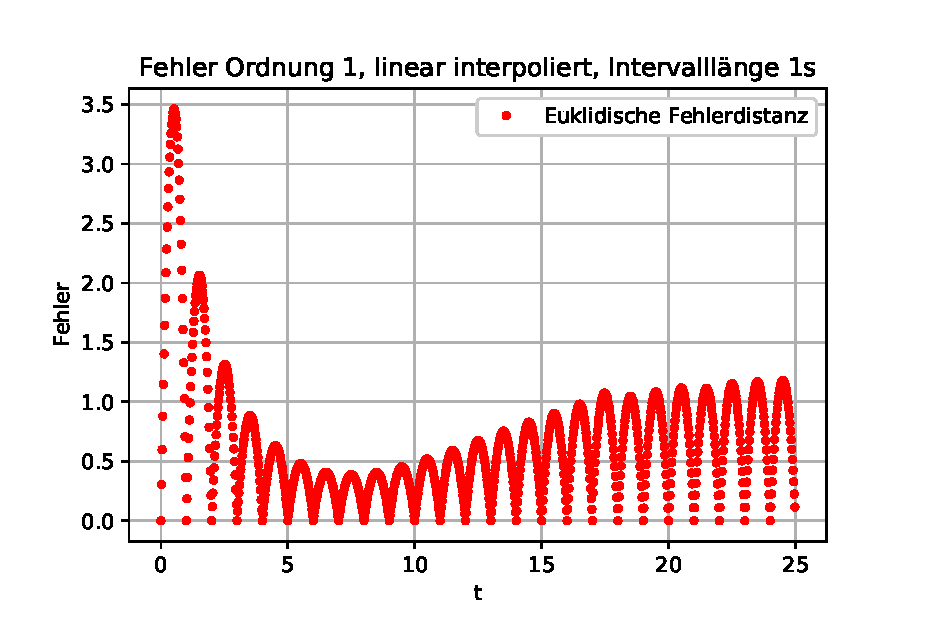
\includegraphics[scale=0.7]{papers/perturbation/bilder/perturbation_fig6.eps}
	\caption{Fehler bei Polynomen erster Ordnung}
	\label{fig:ordnung1_linear_error_A}
\end{figure}

\begin{figure}
	\centering
	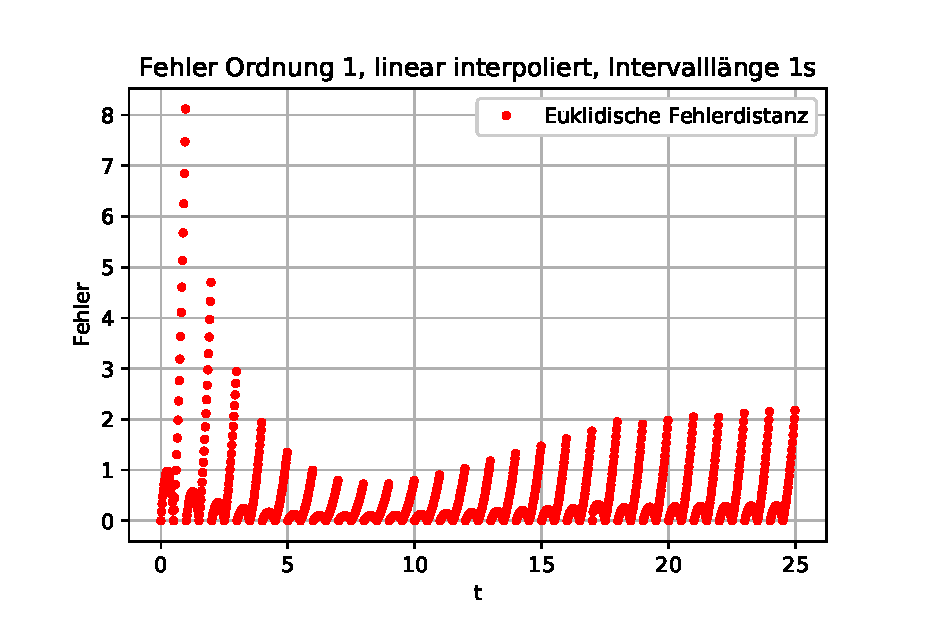
\includegraphics[scale=0.7]{papers/perturbation/bilder/perturbation_fig7.eps}
	\caption{Fehler bei Polynomen erster Ordnung mit variierten Stützstellen}
	\label{fig:ordnung1_linear_error_B}
\end{figure}

\begin{figure}
	\centering
	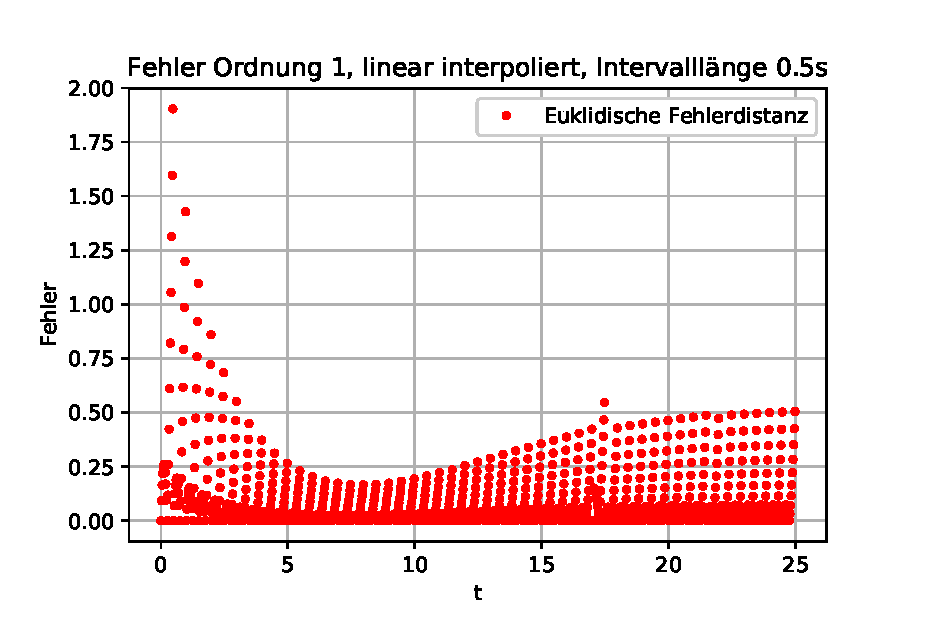
\includegraphics[scale=0.7]{papers/perturbation/bilder/perturbation_fig8.eps}
	\caption{Fehler bei Polynomen erster Ordnung mit halbierter Intervalldauer}
	\label{fig:ordnung1_linear_error_C}
\end{figure}

\subsubsection{Lösung des Problems mit Taylorreihen}
Anstelle von linearer Interpolation, kann man die Unbekannten $r_{x0}, r_{x1}, r_{y0}, \dots$ auch mit anderen Verfahren bestimmen. 
Wir können den Ansatz \eqref{eq:ordnung1_linear_ansatz} als Taylorentwicklungen interpretieren. 
Betrachten wir nur die Ortskoordinate und leiten wir diese nach $\Delta t$ ab, erhalten wir das folgende System. Um die Notation kurz zu halten, verwenden wir Vektornotation anstelle der Aufteilung nach $x$- und $y$-Komponenten.

\begin{equation}
\label{eq:ordnung1_taylor_ansatz}
\begin{aligned}
\vec{r} = & \vec{r_0} + \vec{r_1} \cdot \Delta t \\
\vec{\dot{r}} = & \vec{r_1} \\
\end{aligned}
\end{equation}

Die Unbekannte $\vec{r_0}$ ist erneut durch setzen von $\Delta t = 0$ sehr einfach zu erlangen, analog zu Kapitel \ref{section:perturbation_ordnung1_linear}. $\vec{r_1}$ kann ebenfalls ohne grossen Aufwand bestimmt werden, indem wir die Ableitung mit Hilfe der Bodenstation wie folgt annähern:
\[
\vec{\dot{r}}(t) \approx \frac{\vec{r}(t+\epsilon) - \vec{r}(t)}{\epsilon}
\]

Damit ist bereits eine Annäherung des Ortes möglich. Analog könnte man auch die Geschwindigkeit betrachten.

Beide Varianten, Interpolation und Taylorentwicklung, sind legitim. Die Interpolation ist am Anfang und Ende des Intervalles exakt, hat dafür aber in der Mitte einen relativ hohen Fehler. Die Taylorentwicklung ist vor allem zu Beginn des Intervalls exakt. Dies, da insbesondere bei höheren Ordnungen auch die Krümmung des Kurvenverlaufs berücksichtigt wird. Da sich allerdings alle Stützstellen am Anfang des Intervalles befinden, wird der Kurvenverlauf zum Ende des Intervalles hin immer ungenauer.
